\documentclass{article}

\usepackage{lipsum}
\usepackage[margin=4cm, includefoot]{geometry}
\usepackage{graphicx}
\usepackage{float}
\usepackage{indentfirst}
\usepackage{listings}
\usepackage{hyperref}
\usepackage{color}

% Header and footer
\usepackage{fancyhdr}
\pagestyle{fancy}

\rhead{}
\lhead{}
\fancyfoot{}
\fancyfoot[R]{\thepage}
\renewcommand{\headrulewidth}{0pt}
\renewcommand{\footrulewidth}{0pt}
%

\begin{document}

\begin{titlepage}
	\begin{center}
		\line(1,0){400}\\
		[6mm]
		\huge{\bfseries User Manual}\\
		\line(1,0){400}\\
		[5mm]
		
\includegraphics[width=150px]{../images/AWorldOfPlants.png}
		\\
		[5mm]
		\large\textbf{Project:}\\A World of Things\\
		[3mm]
		\large\textbf{Client:}\\Julian Hambleton-Jones\\
		[3mm]
		\large \textbf{Team:}\\Funge\\
		\line(1,0){400}\\
		[5mm]
		\large \textbf{Team Members:}\\
		[3mm]
		\large 14214742 - Matthew Botha\\
		\large 14446619 - Gian Paolo Buffo\\
		\large 14027021 - Matthias Harvey\\
        \large 14035538 - Dillon Heins\\[3mm]
	\end{center}
\end{titlepage}

\cleardoublepage
\thispagestyle{empty}
\tableofcontents
\begin{table}[]
\centering
\caption{Version Table}
\label{my-label}
\begin{tabular}{|l|l|l|ll}
\cline{1-3}
\textbf{Version} & \textbf{Date} & \textbf{Description}                                                                                                                                                                                                               &  &  \\ \cline{1-3}
0.1              & 22/05/2016    & \begin{tabular}[c]{@{}l@{}}Vision, scope, architectural requirements\\ and initial architecture design.\end{tabular}                                                                                                               &  &  \\ \cline{1-3}
0.2              & 29/07/2016    & \begin{tabular}[c]{@{}l@{}}Creation of separate documents for architecture\\ design, software requirements, testing and user \\ manual. Each populated with the relevant\\ information for the project at this stage.\end{tabular} &  &  \\ \cline{1-3}
0.3              & 11/09/2016    & \begin{tabular}[c]{@{}l@{}}Remake of all documents. Combination of them\\ into a single document. Documents follow\\ guidelines as discussed with lecturer.\end{tabular}                                                           &  &  \\ \cline{1-3}
\end{tabular}
\end{table}
\cleardoublepage
\setcounter{page}{1}

\textit{Disclaimer: The system is still under development. All documentation will be updated as the system progresses}

\section{System Overview}
	A World of Plants makes use of networked hardware devices to allow users to use the Internet to monitor and control the environment of living plants in real time.
	
	The system has been designed to make independent agriculture a fun and personalised experience. Compete to unlock new rewards or progress at your own leisure. Follow the plant suggestions to-the-letter or follow your own intuition. It's all up to you.
	
	Welcome to A World of Plants.

\section{System Configuration}
	A World of Plants is made up of 3 distinct parts:
	\begin{itemize}
		\item \textbf{Plant Box}, where your plants will live and grow. Your sensors will sit here as well.
		\item \textbf{The Cloud}, where all the behind-the-scenes magic takes place. Without this, there would be no data persistence, storage or communication.
		\item \textbf{Web app}, which you'll use to view plant info, interact with plants, and see how far you're progressing.
	\end{itemize}
	
	\begin{figure}[H]
		\includegraphics[width=\textwidth]{../images/UserManual/plant-box.png}
		\caption{Plant Box}
	\end{figure}
	
	\begin{figure}[H]
		\includegraphics[width=\textwidth]{../images/UserManual/the-cloud.png}
		\caption{The Cloud}
	\end{figure}
	
	The rest of the User Manual focuses on the Web app.
\section{Installation}
	\subsection{User Installation}
		The software can be found at \url{http://www.funge.cf}
		
		There is no installation necessary if you are an ordinary user, it is as simple as visiting the above listed website and registering.
		
		Registration can be done as follows:
		\begin{itemize}
			\item Visit \url{http://funge.cf}
			\item Select "Need an Account?"
			\item Enter the relevant details
			\item After selecting the "Sign Up" button you should be logged in automatically
		\end{itemize}
	
	\subsection{Software Developer Installation}
		The software can be found at \url{https://github.com/DillonHeins/Funge}
		\subsubsection{Initial Set Up}
			\begin{itemize}
				\item Set up an AWS account by visiting:
					\begin{itemize}
						\item \url{https://aws.amazon.com/}
					\end{itemize}
				\item Download and install the AWS command line interface:
					\begin{itemize}
						\item Additional information can be located at \url{https://aws.amazon.com/cli/}
					\end{itemize}
				\item Install Java Development Kit 8:
					\begin{itemize}
						\item \url{http://www.oracle.com/technetwork/java/javase/downloads/jdk8-downloads-2133151.html}
					\end{itemize}
				\item Install Apache Maven. Instructions on how to download, install and run Maven can be located at:
					\begin{itemize}
						\item \url{https://maven.apache.org/}
					\end{itemize}
			\end{itemize}
		\subsubsection{Java Backend Installation}
			\begin{itemize}
				\item Navigate to BackEnd/a-world-of-plants
				\item Open a command line window on your operating system of choice
				\item Run the command:
				\begin{itemize}
					\item 
\begin{lstlisting}
mvn test package
\end{lstlisting}
					\item This command will first test the code to ensure it is running accordingly and it will then package the software into a .jar file
				\end{itemize}
				\item Navigate to BackEnd/a-world-of-plants/target
				\item In order to upload the .jar to AWS S3 and deploy it to AWS Lambda run the following commands:
					\begin{itemize}
						\item 
\begin{lstlisting}
aws s3 cp jarname.jar s3://bucket-name
\end{lstlisting}

						\item
\begin{lstlisting}
aws lambda update-function-code --function-name function 
\--s3-bucket bucket-name --s3-key jarname.jar
\end{lstlisting}
					\end{itemize}	
			\end{itemize}
		\subsubsection{AngularJS Frontend Installation}
			Navigate to FrontEnd/AWorldOfPlantsApp
			\begin{itemize}
				\item To run the AngularJS App locally:
					\begin{itemize}
						\item Open a command line interface on your operating system of choice
						\item Run the command:
							\begin{itemize}
								\item 
\begin{lstlisting}
npm install
\end{lstlisting}
							\end{itemize}
						\item Navigate to http://localhost:8000 in your browser
					\end{itemize}
				\item To deploy the AngularJS App to S3 run the command:
					\begin{itemize}
						\item
\begin{lstlisting}
aws s3 cp app s3://website.com --recursive --exclude "*.log"
\end{lstlisting}
					\end{itemize}
			\end{itemize}		

\section{Getting Started}

\section{Using the System}

\section{Troubleshooting}
	The system has been designed to return varying HTTP status codes depending on whether an operation was successful or not. If a user would like to see more detail with regard to these codes they may open the developer console on their preferred browser. However, the system automatically responds to these codes and handles them accordingly.\\
	
	The details of these HTTP status codes are listed below:
	\begin{itemize}
		\item 200 - success
			\begin{itemize}
				\item This is the code returned when all operations are functioning as expected
				\item The system should continue without any problems or user intervention
			\end{itemize}
		\item 400 - client error
			\begin{itemize}
				\item This code is associated with bad requests
				\item A bad request occurs whenever a request fails validation, i.e. when a client formats the request in a manner that the system was not expecting
				\item This could occur when the user enters incorrect details or when a page is requested that does not exist
			\end{itemize}
			\begin{figure}[H]
				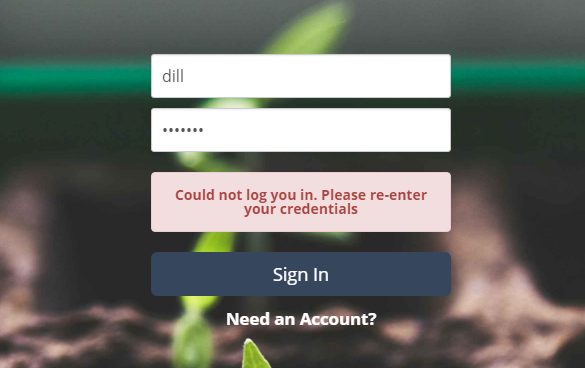
\includegraphics[width=\textwidth]{../images/UserManual/400error.png}
				\caption{Incorrect User Details Error}
			\end{figure}
		\item 500 - server error
			\begin{itemize}
				\item This occurs when an internal error occurs on the server. The server will attempt to resolve this issue without user intervention as best as possible.
				\item The user may be notified if the error affects them
			\end{itemize}
			\begin{figure}[H]
				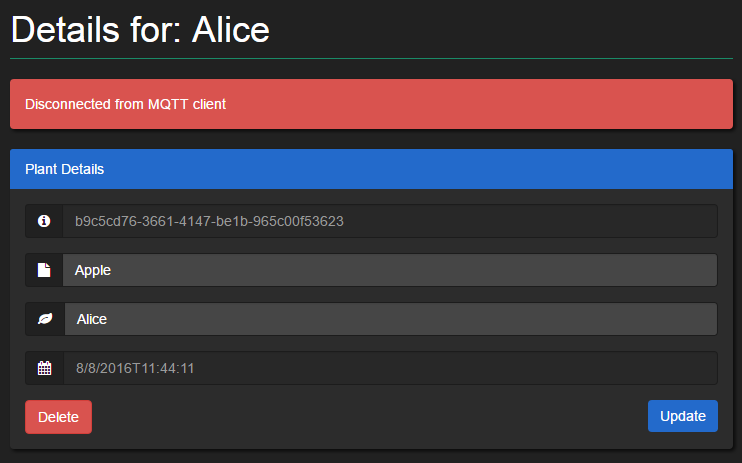
\includegraphics[width=\textwidth]{../images/UserManual/500error.png}
				\caption{Error Establishing Connection to Plant Box}
			\end{figure}
	\end{itemize}

\section{Landing Page}
	\subsection{Logging in}
		\textcolor{red}{(1)} The first page you'll encounter is the login page. If you already have an account, enter your username and password in the appropriate blocks and click "Sign In".
		\newline
		\textcolor{red}{(2)} If you'd like to find out more about A World of Plants, you can scroll down to our information page. Scroll back up when you're ready to login or register.
		\newline
		\textcolor{red}{(3)} If you have not yet registered, click on "Need an account?" to navigate to the account registration.
		\begin{figure}[H]
			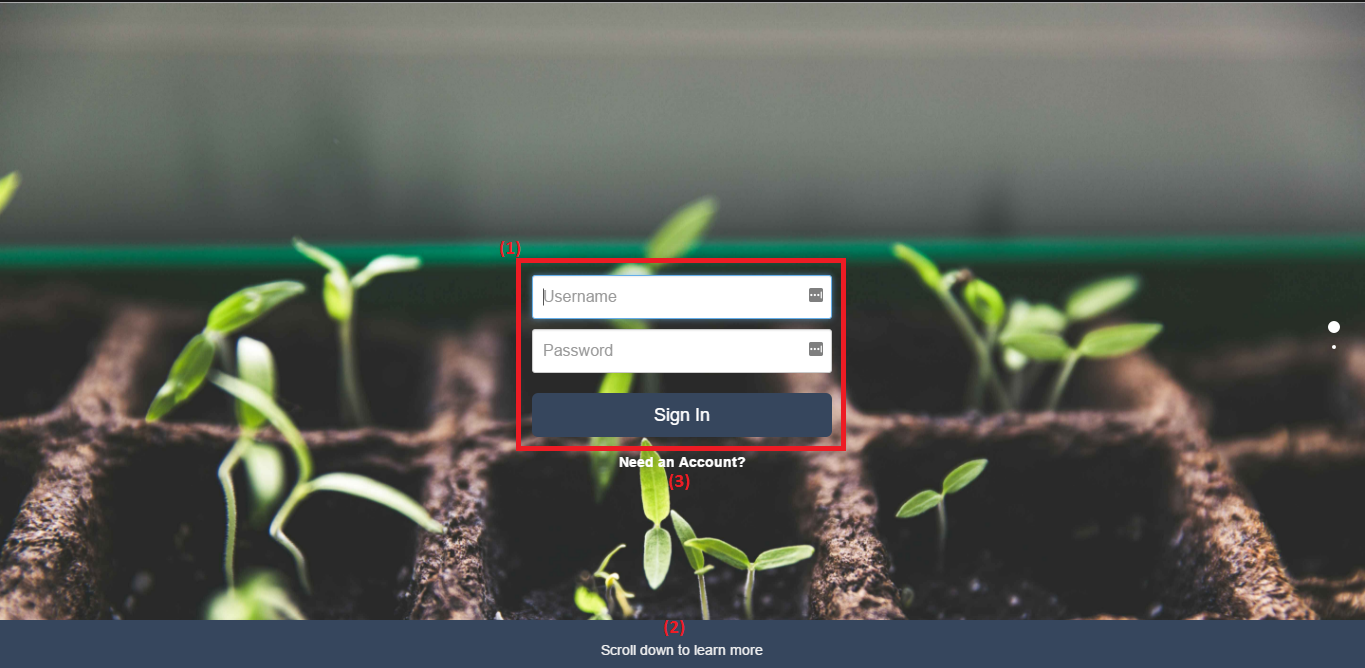
\includegraphics[width=\textwidth]{../images/UserManual/login.PNG}
			\caption{Login Page}
		\end{figure}				
		
	\subsection{Account Registration}
		\textcolor{red}{(1)} If you do not yet have an account, enter your email, the username you'd like to be known by, and your password (twice) and click the "Sign Up" button.
		\newline
		\textcolor{red}{(2)} If you already have an account and would like to log in, click on "Have an Account?" to navigate to the user login.
		\newline
		\begin{figure}[H]
			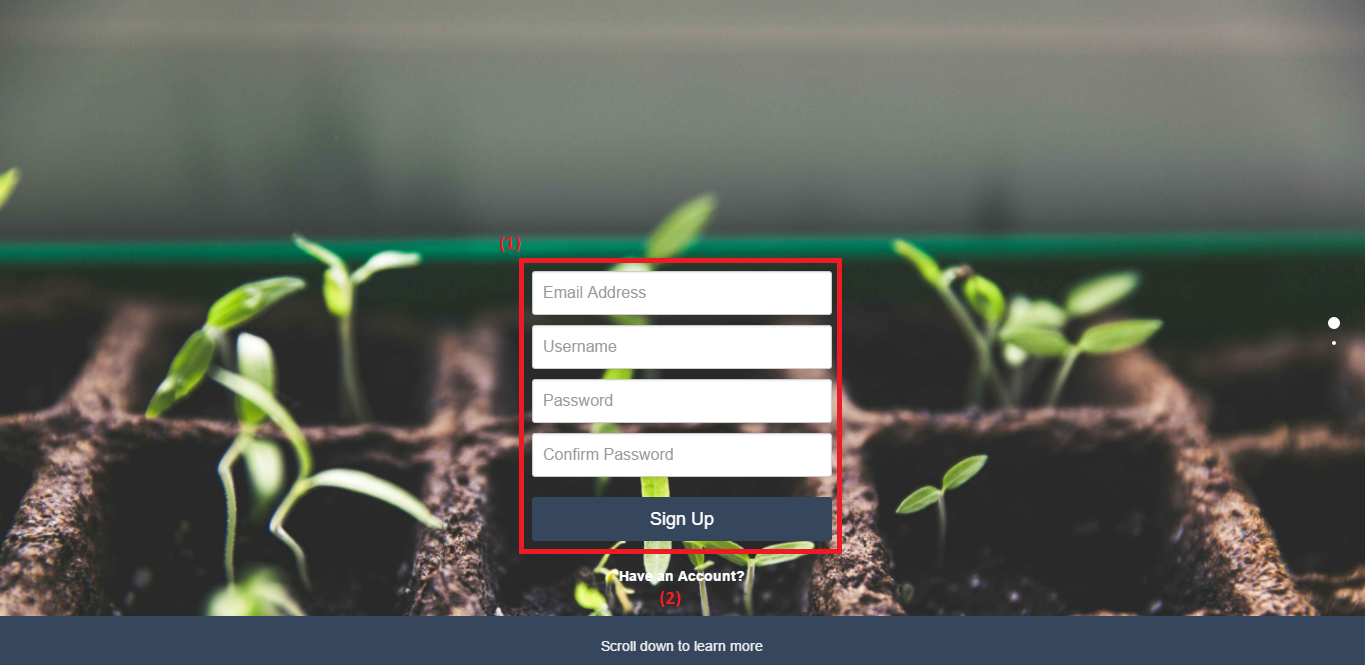
\includegraphics[width=\textwidth]{../images/UserManual/registration.PNG}
			\caption{Registration Page}
		\end{figure}
		
\section{Main Site}
	\subsection{Navbar}
	All pages on the main site will display the navbar at the top.
		\subsubsection{User Actions}
		\textcolor{red}{(1)} To access your user actions, click on your username at the right of the navbar. From here, you can either navigate to your profile or log out.
		\begin{figure}[H]
			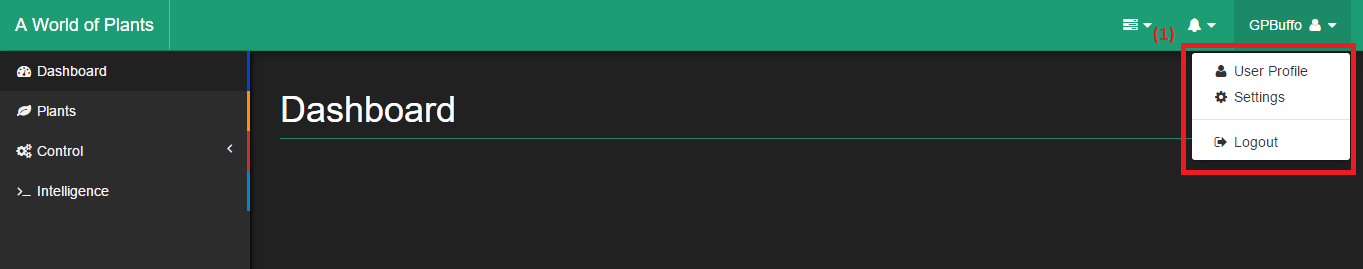
\includegraphics[width=\textwidth]{../images/UserManual/navbar-user-actions.PNG}
			\caption{Navbar User Actions}
		\end{figure}
		
	\subsection{Plants}
	To access your plants, click on "Plants" in the sidebar. This page will display a summary of all your current plants.
	\newline
	\textcolor{red}{(1)} To add a new plant, click on the "Create New Plant" button on the top right. See \hyperref[sec:creating-a-plant]{Creating a Plant} for more information.
	\newline
	\textcolor{red}{(2)} To view more information or change some of the details for a specific plant, click on "View Details" for the plant of your choice. See \hyperref[sec:plant-details]{Plant Details} for more information.
	\begin{figure}[H]
		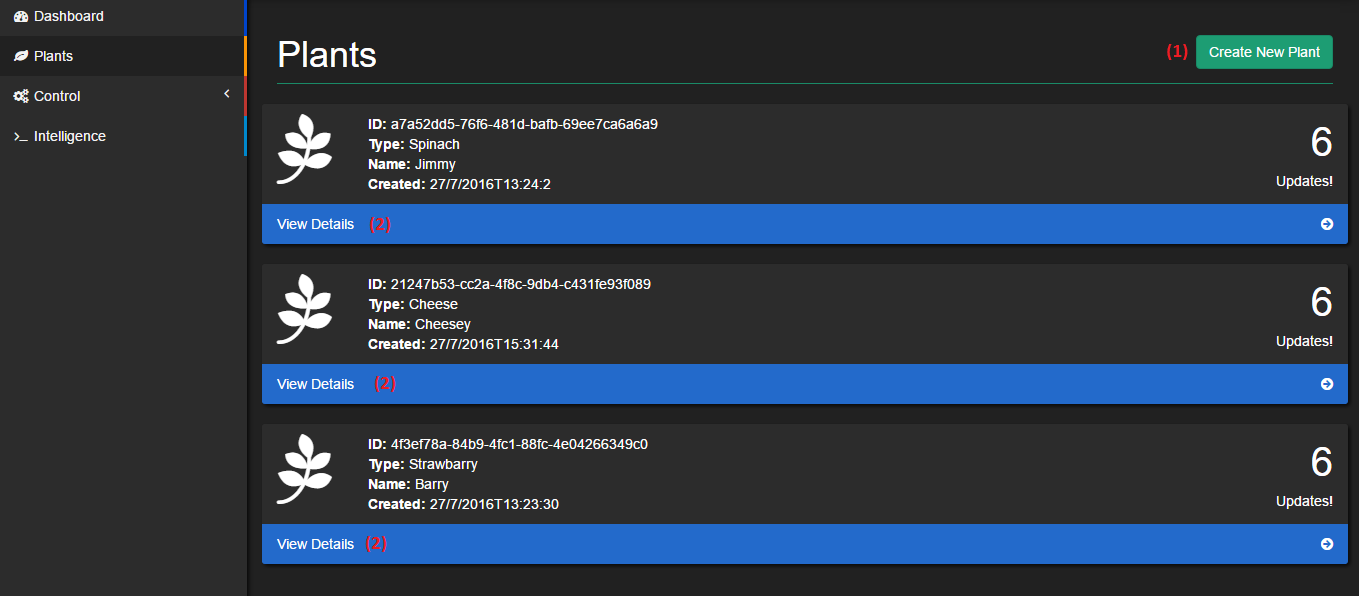
\includegraphics[width=\textwidth]{../images/UserManual/plants.PNG}
		\caption{Plants View}
	\end{figure}
		
		\subsubsection{Creating a Plant}
		\label{sec:creating-a-plant}
		To create a plant, enter the plant's unique details and then click on "Create".
		\begin{figure}[H]
			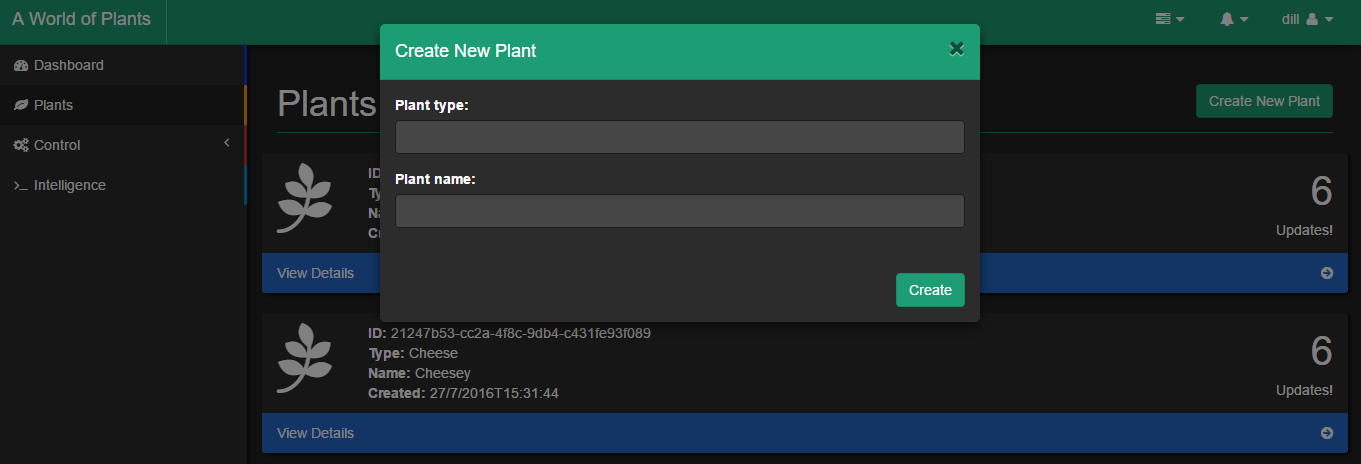
\includegraphics[width=\textwidth]{../images/UserManual/create-plant.PNG}
			\caption{Creating a Plant}
		\end{figure}
		
	\subsection{Plant Details}
	\label{sec:plant-details}
	From here you can get an overview of all of your plant's details.
	\newline
	\textcolor{red}{(1)} To update plant details such as the plant's name or category, make your desired changes and then click the "Update" button.
	\newline
	\textcolor{red}{(2)} If you'd like to delete your plant, click on the red "Delete" button. \textbf{This is permanent}, so be careful.
	\begin{figure}[H]
		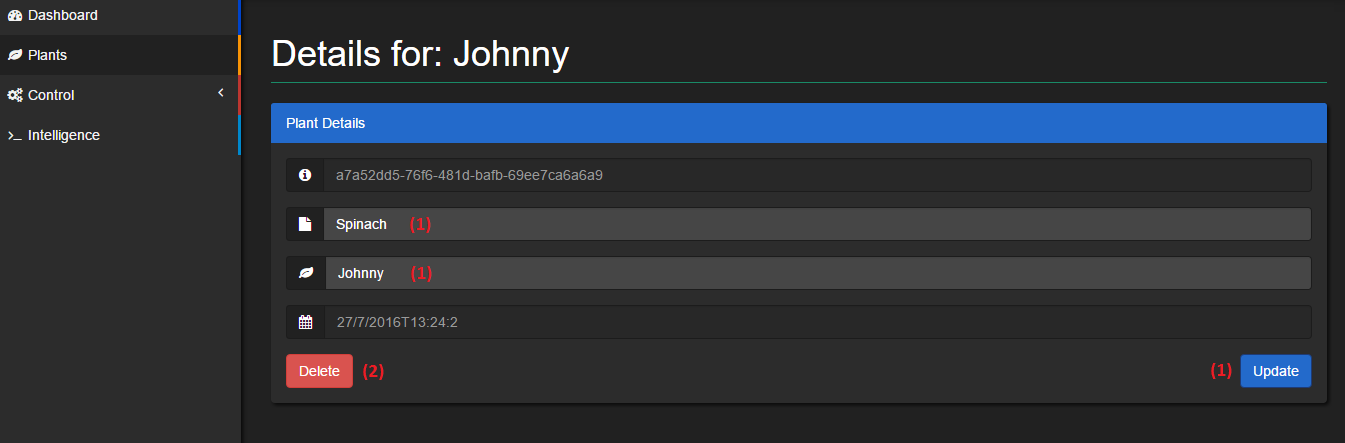
\includegraphics[width=\textwidth]{../images/UserManual/plant-details.PNG}
		\caption{Plant Details}
	\end{figure}

\end{document}